
        \documentclass[tikz]{standalone}
        \begin{document}
        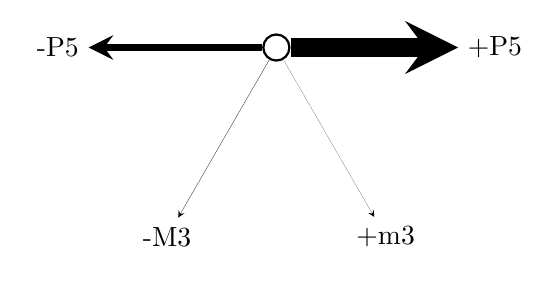
\begin{tikzpicture}[scale=3.5, ->, >=stealth]

        % the circle
        \node (origin) at (0,0) [draw,circle,black,fill=white,thick]{};
        % constant scaling for widths
        \def\cons{10}
        
                \node (0) at +(0*360/6:0.7929325023383746) {+P5};
                \path (origin) edge [line width=\cons*0.7056695217453453] node {} (0);
                
                \node (1) at +(-1*360/6:0.7929325023383746) {+m3};
                \path (origin) edge [line width=\cons*0.0016927144274005534] node {} (1);
                
                \node (2) at +(-2*360/6:0.7929325023383746) {-M3};
                \path (origin) edge [line width=\cons*0.009093129016023672] node {} (2);
                
                \node (3) at +(-3*360/6:0.7929325023383746) {-P5};
                \path (origin) edge [line width=\cons*0.2835446348112306] node {} (3);
                
        \end{tikzpicture}
        \end{document}
        